 
\chapter{Spreadsheets}


\section{Libr\'{e} Office Calc}
\label{sec:calc}

\subsection{Introduction}


Spreadsheets were one of the original ``killer apps'' when personal computers were first introduced.  Spreadsheets allow you to deal with tables of numbers and other data.  The standard convention is that the rows of a spreadsheet are indexed by numbers and the columns are indexed with letters.  If you need to go past 26 columns, use AA, AB, AC, {\em et cetera} for the next several columns.  It would be pretty unusual to need to have more than 702 columns but if you needed to, guess what comes after ZZ.

We're going to be using the free/open-source Libr\'{e} Office spreadsheet in the upcoming labs.  There are other choices (Excel on Windows and Numbers on Apple computers) but all of them work in a similar way and Libr\'{e} Office is free.  Spreadsheet files created by 
Libr\'{e} Office have a .ods suffix.  

To load Libr\'{e} Office on your personal machine, visit \url{https://www.libreoffice.org/download/download-libreoffice/}

In the next lab, you're going to need the formula for simple interest.  Interest is a slightly funny concept -- it comes from the idea that there is value in posessing some amount of money (you can invest it to make more money, or you can spend it in ways that are enjoyable\dots)  So, when one person loans money to another, the receiving party should pay them back ``a little bit extra'' to compensate them for the loss of the use of their funds.  That ``little bit extra'' is called interest.  The simplest possibility would be for interest to be just a uniformly fixed amount -- say \$10.  But that would be pretty unfair in some situations.  If I borrowed \$2 from a friend to buy a coffee, should I really pay them back \$12 the next day?  At the other end of the scale, if a business borrows \$1,000,000 from a bank, does it seem fair that they'd have to repay
\$1,000,010 five years later?

It seems pretty clear that interest should (at least) depend on two things:  the amount borrowed, and the duration of the loan.  In the simple interest formula, these things are typically called $P$ (the \underline{principal}) and $t$ (the \underline{time} -- usually measured in years).  The other element we'll need is called the \underline{rate}, which 
is usually called $r$ and expressed as a percentage.  When $r$ (which must be agreed upon by the two parties) is given as a percentage, we must convert it to a decimal to use it in the formula (for example $6\%  = 0.06$) 

With all that as prelude, the interest $I = Prt$ and the amount to be repaid is $A = P + I$, which can be re-expressed as 

\[ A \; = \; P + Prt \; = \; P \cdot (1 + rt). \]

\noindent This is known as the simple interest formula.

\clearpage
\begin{worksheet}{11}{Intro to Spreadsheets}{LibreCalc.png}
If you haven't done so already, visit \url{https://www.libreoffice.org/download/download-libreoffice/} and download the Libr\'{e} Office suite.

Suppose a businessman was in the completely legitimate business of making loans to people who are regarded as poor credit risks by conventional banks.  Of course, he'd want to keep track of the loan amounts and the recipients.  A spreadsheet is the perfect tool!

Here's a screen shot of how the data might be recorded:

\centerline{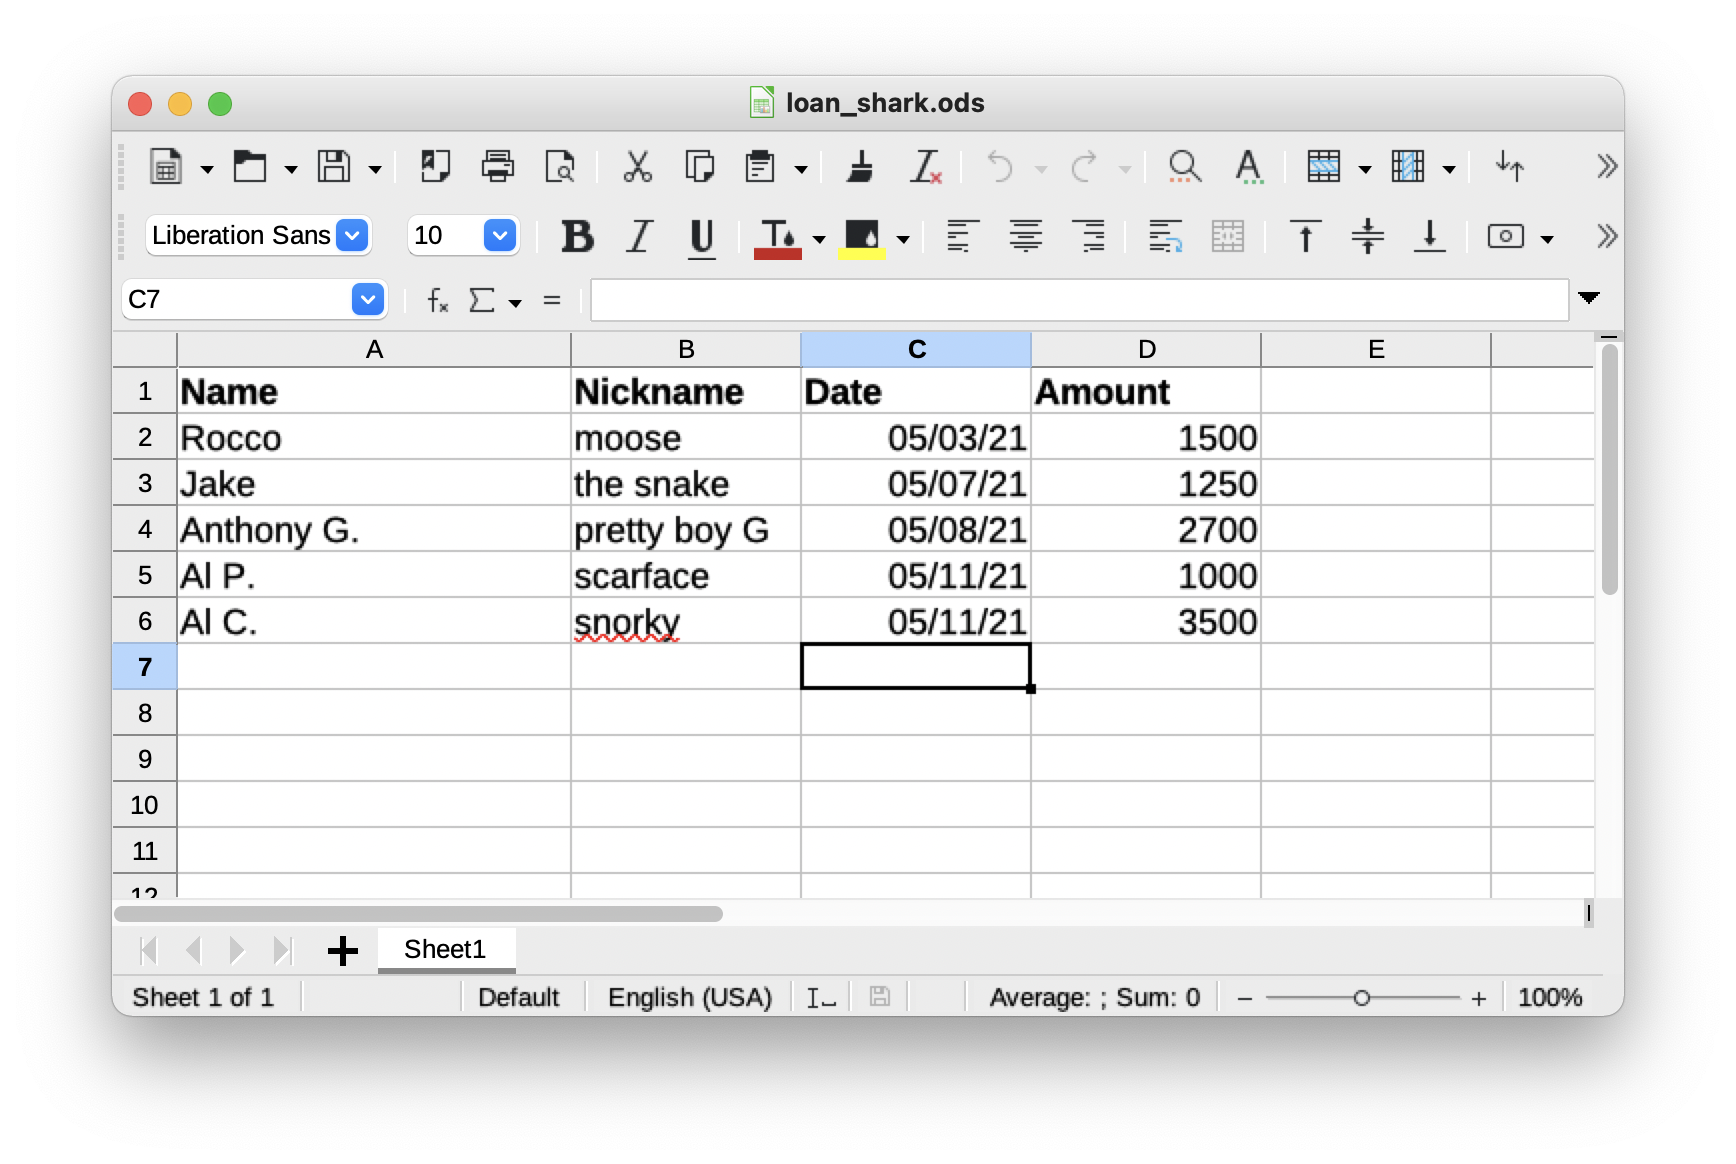
\includegraphics[scale=.5]{loans.png}}

We're using the free/open-source Libr\'{e} Office spreadsheet in the above.  There are other choices (Excel on Windows and Numbers on Apple computers) but all of them work in a similar way and Libr\'{e} Office is free.  Spreadsheet files created by Libr\'{e} Office have a .ods suffix.  

The stuff that you enter into a cell in a spreadsheet fall into two main categories: a cell can contain data, or a cell can contain a calculated value.  To make a ``calculation''-type cell you have to put an equals sign up front.  When you're doing a calculation you can use the values that are in other cells by referring to them by column (letter) followed by row (number).  For example the \$3500 that Snorky borrowed is in cell D6.

Some calculated cells are pretty simple, like the sum, difference or product of the values in other cells.
Other calculated cells can be pretty complex -- there are a lot of built-in functions that can be used to do these more difficult computations.  Once you know your way around, you'll probably just type the name of the function you need.  Until then there is the so-called ``function wizard.''  Try looking for a function that will give you random numbers.

\centerline{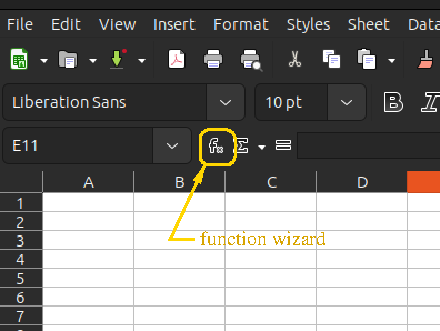
\includegraphics[scale=.5]{func_wiz.png}}

\subsubsection{tasks}

\begin{enumerate}

\item Open the loan shark spreadsheet (the file is available on the book website) and make some additions -- columns for monthly interest rate, due date and the current amount due.  You should verify that subtracting the values in two cells that are formatted as dates does the right thing.  Since you'll want time to be measured in months, what conversion needs to be applied?

\item Create a spreadsheet for keeping track of student grades in a math class. Use your favorite actors, sports stars, musicians (or whatever) as students, and just generate random numbers to put in as their grades. Make the homework grades (let's say 5 different scores) be on a scale from 0 to 10.  Make the quiz grades (also 5 of them) be on a scale from 0 to 20. Finally, make up two exam scores on a 0 to 100 scale.
Create subtotals for homework, quizzes and exams, also a grand total with homework weighted $20\%$, quizzes weighted
$30\%$ and exams weighted $50\%$.  

Many teachers have policies where the lowest grade in some category is dropped.  Figure out how to drop the lowest quiz score.

\end{enumerate}


\end{worksheet}
\clearpage


\subsection{Absolute and relative cell references}

\subsubsection{tech}

If you're going to be using the same calculation in a bunch of different places, you can just copy and paste the contents of one cell into another.  Get used to using the keyboard shortcuts Ctrl-C and Ctrl-V for copy and paste.  

When you copy and paste a formula, the spreadsheet intelligently changes the cell references in the formula.  The pasted formula refers to cells that are in the same positions {\em relative} to the spot we're pasting into.  

For example, if you type {\tt =B3 + C2}  into cell {\tt C3} you're telling the system to add the number just above and the number just to the left.  If you copy and paste that formula into cell {\tt K7} you'll find that the formula has become {\tt =J7+K6} because those cells are in the same relative positions.

This intelligent pasting {\em usually} does the right thing, but occasionally we really just want the thing to stay put!  If you want a cell reference to {\em not} change when you're cutting and pasting (this is known as an absolute reference) put dollars (\$) in front of both the letter and the number.  Very occasionally we want a sort of hybrid behavior -- we can put the dollar on one but not the other.  For instance, if in a formula we refer to a cell using \$A3  (with the dollar on the A but not in front of the 3) when we copy and paste the A will stay an A, but the 3 will change appropriately.  Some people call this making either the row or the column ``sticky.''  

\subsubsection{math}

In today's activity we'll be looking at two mathematical concepts: binomial coefficients and difference tables.

Binomial coefficients are sometimes called {\em choice counters}.  For example, given a set of 5 options how many ways can we select 3 of them?  This would be the binomial coefficient $\binom{5}{3}$ which is equal to 10.  To pronounce that symbol in English use the word ``choose,''  so the symbol above is read as ``five choose three.''  That notation for binomial coefficients can be a little confusing since many people assume the fraction bar just got left off!  So be careful, $\binom{5}{3} \; = \; 10$, but $\left( \frac{5}{3} \right) \; = \; 1.666\ldots$  so (obviously) these are different -- don't imagine fraction bars where they don't actually appear!

There is another notation for the same quantities using a capital letter $C$.  To indicate ``five choose three'' in this notation write $_5C_3$.

So why are these choice counters called ``binomial coefficients''?   It turns out these numbers also appear when taking powers of a {\em binomial} -- a polynomial with just two terms.  Try computing $(x+1)^0$, $(x+1)^1$, $(x+1)^2$ and $(x+1)^3$.  Really, only the last of those is at all difficult!  Anything to the $0$ power is just $1$, anything to the $1$ power is itself, and the $2$nd power just requires the FOIL rule!

Blaise Pascal -- a French mathematician who was one of the founders of the field of probability -- was probably the first to notice the pattern when you write these things next to one another.


\begin{tabular}{c}
	$1$ \\
	$x+1$ \\
	$x^2+2x+1$ \\
	$x^3 + 3x^2 + 3x+1$\\
\end{tabular}

The pattern becomes easier to deduce if you remove all the powers of $x$ (and the plus signs) and just concentrate on the coefficients.

\begin{tabular}{c}
	$1$ \\
	$1 \quad 1$ \\
	$1 \quad 2 \quad 1$ \\
	$1 \quad 3 \quad 3 \quad 1$\\
\end{tabular}

 Numbers on the outside of each row are always 1.  Numbers in the middle of a row are just the sum of the two things above them.
 
 The arrangement of binomial coefficients into this triangular array is called Pascal's triangle.  Here's the first 5 rows:
 
 \begin{tabular}{c}
 	$1$ \\
 	$1 \quad 1$ \\
 	$1 \quad 2 \quad 1$ \\
 	$1 \quad 3 \quad 3 \quad 1$\\
 	$1 \quad 4 \quad 6 \quad 4 \quad 1$\\
 	$1 \quad 5 \quad 10 \quad 10 \quad 5 \quad 1$\\
 \end{tabular}
 
 Difference tables come from a very common form of analyzing a sequence.
 
 Suppose we asked, ``What comes next?'' in the following sequence.
 
 \[ 4, \quad 7, \quad 10, \quad 13, \ldots \]
 
 You probably notice rather quickly that successive terms in the sequence differ by the same number.  A difference table is just a formalized way of making the same observation -- except that if the differences don't seem to have an obvious pattern we might continue on taking the differences of the differences!
 
 Here's an example.  Suppose you're given the following sequence of numbers.
 
 \[ 2 \quad 5 \quad 12 \quad 23 \quad 38 \quad \ldots \]
 
 A difference table looks like so:
 
 \begin{tabular}{ccccccccc}
 	2 &  & 5 & & 12 & & 23 & & 38 \\
 	   & 3 & & 7 & & 11 & & 15 
 \end{tabular}

Since the differences don't exhibit an obvious pattern we continue on, obtaining

\begin{tabular}{ccccccccc}
	2 &  & 5 & & 12 & & 23 & & 38 \\
	& 3 & & 7 & & 11 & & 15 & \\
	& & 4 &  & 4  &  & 4 & & \\ 
\end{tabular}

It looks as though the bottom row -- which is known as the {\em second differences} is always 4.  Can you use that to predict what the next term in the sequence will be?

\clearpage
\begin{worksheet}{12}{More on Spreadsheets}{LibreCalc.png}
\begin{enumerate}

\item Write out the expanded form of $(x+1)^5$. (You may want to open a Sage session for this.)

\vspace{1in}

\item Use a spreadsheet to create a table of the binomial coefficients $\binom{n}{k} = \frac{n!}{k!(n-k)!}$.  The rows in the table should be left-justified, for instance, column A will contain all of the $1$'s that form the first entries of the rows.  You should create your table twice.  Once using the builtin function $\tt COMBIN()$ (look for it in the function wizard) -- you'll need to think carefully about what should be ``sticky'' in this case!  The second version of the table should use the rule that the entries in Pascal's triangle are the sum of the ones above and on either side of them -- here, you'll need to think carefully about how ``on either side'' morphs when the table is left-justified.
	

\vspace{1in}

\item Revisit the grade spreadsheet from the previous section and insert a new row at the top.  Put the "weights" for homework, 
quizzes and exams into cells in this row.  (As the teacher you might want to experiment with different 
weighting schemes.) Are the final grades changed by much if we change the weights to 10, 
20 and 70 percent respectively?

\vspace{1 in}

\item Use a spreadsheet to do a finite differences analysis of the following sequence:

	  \[ 1 \quad 3 \quad 7 \quad 13 \quad 21 \ldots \]

\vspace{1in}

\item Find the "back diagonals" for the sequences of squares, cubes, 4th  and 5th powers.
(We care about back diagonals because you can use them to generate the entire sequence! (under the assumption that the bottom-most number is a constant) (sorry about all the parentheses)). 

\vfill

\end{enumerate}

\end{worksheet}
\clearpage



\subsection{Builtin functions}


\clearpage
\begin{worksheet}{13}{Spreadsheets: Built-in functions}{LibreCalc.png}
Returning to our gradebook example$\ldots$

On the TFLabs website, find and download the file ``grades.ods''

In this spreadsheet, the MIN function has been used to ``drop the lowest quiz.''  Is this how you accomplished this in Lab 11?  The cells that contain weights for the various kinds of assessments are also there, and accessed in the formulas for cells using absolute (a.k.a. sticky) references.

\begin{enumerate}

\item Look up the {\tt CHOOSE()} and the {\tt INT()} functions in the function wizard, and figure out how to use them to assign letter grades with $+$ and $-$ modifiers.

\vspace{1in}

\item There are quite a few ``mathematical'' functions available in the function wizard.  For example, many of the functions that start with `A' are inverse trigonometric functions\dots  Figure out how to use ordinary division and the {\tt FLOOR()} function to find the quotient and reaminder you get when dividing one number by another.

\vspace{1in} 

\item Closely related to questions about the division process, there are two important mathematical functions called {\tt GCD()} and {\tt LCM() }.  Play around with these to discover what they do.  Can you determine a formula for {\tt GCD() $\times$ LCM() }?

\vfill

\end{enumerate}

\end{worksheet}
\clearpage

\subsection{Project Ideas}

{\bf Stocks}

You can get historical data about stock prices from the Yahoo! Finance site.  Go to Yahoo! Finance and search for a company you might be interested in.  Click on the tab labelled historical data and then look for the download link.  The result will be stock price information for the previous year in a CSV file (comma seperated values).  CSVs are sort of the ``lowest common denomenator'' for spreadsheets -- they are readable by all spreadsheet applications.  Analyse the stock prices in an effort to decide if a given day day is a ``buy opportunity.''  (According to the famous adage we should ``buy low and sell high'' so we're looking for days where the price is reasonably low, but we expect it to go up!)  Be careful that you mark buy opportunities strictly on the basis of past information.  If you hope to get rich, but don't have a time machine, that's all you'll have to go on.

\noindent {\bf Mortgages}

There is a mathematical formula for mortgages and there are plenty of online calculators that one can use to determine the monthly payment on a particular house.  Nevertheless, let's see if we can use a spreadsheet to determine the monthly payment for a given loan.  Every month during the life of a mortgage, two competing things are happening:  a month's worth of interest is added to the balance, and the monthly payment is subtracted from the balance. The goal is to choose the monthly payment so that after 240 months (i.e. 20 years) the balance hits 0.

\noindent {\bf Stirling numbers}

You'll need to do some Googling for this one.  There are two kinds of Stirling numbers, which are given the names 
``Stirling numbers of the first kind'' and ``Stirling numbers of the second kind.''  Both are computable because they satisfy recursions similar (but a bit more complicated) than the binomial coefficients.  Use a spreadsheet to create tables of both kinds of Stirling numbers.  Both of these sets of numbers numbers solve unusual counting problems, do some research and explain what they're for to us.

\noindent{\bf acciones en una empresa}
Puede obtener datos históricos sobre los precios de las acciones en Yahoo! Sitio de finanzas. Ir a Yahoo! Financia y busque una empresa que pueda interesarle. Haga clic en la pestaña denominada datos históricos y luego busque el enlace de descarga. El resultado será información sobre el precio de las acciones del año anterior en un archivo CSV (valores separados por comas). Los CSV son una especie de "mínimo común denominador" para las hojas de cálculo: son legibles por todas las aplicaciones de hojas de cálculo. Analice los precios de las acciones en un esfuerzo por decidir si un día determinado es una "oportunidad de compra". (Según el famoso adagio debemos "comprar barato y vender caro", por lo que buscamos días en los que el precio es razonablemente bajo, ¡pero esperamos que suba!) Tenga cuidado de marcar las oportunidades de compra basándose estrictamente en información pasada. Si esperas hacerte rico, pero no tienes una máquina del tiempo, eso es todo lo que tendrás que hacer.